\documentclass[12pt,twoside]{reedthesis}
\usepackage{graphicx,latexsym} 
\usepackage{amssymb,amsthm,amsmath}
\usepackage{longtable,booktabs,setspace} 
\usepackage{url}
\usepackage{natbib}
\usepackage{algorithm}
\usepackage{algorithmic}

\title{My Final College Paper}
\author{Ivan A. Malison}
\date{April 2012}
\division{Mathematics and Natural Sciences}
\advisor{James D. Fix}

\department{Mathematics}


\setlength{\parskip}{0pt}
\begin{document}

  \maketitle
  \frontmatter 
  \pagestyle{empty}

  \chapter*{Acknowledgements}

    \chapter*{Preface}

    \tableofcontents

    \chapter*{Abstract}
	
	\chapter*{Dedication}

  \mainmatter 
  \pagestyle{fancyplain}

    \chapter*{Introduction}
         \addcontentsline{toc}{chapter}{Introduction}
	\chaptermark{Introduction}
	\markboth{Introduction}{Introduction}

\chapter{GPU Hardware}

The following chapter describes the basic design of modern GPUs and the factors that informed these design decisions.
%%Though the architectural features highlighted in this section will inform the development of algorithms developed later in the paper, keep in mind that this description is a something of a cartoon, and that actual GPU hardware is usually more sophisticated.

\section{The Graphics Pipeline}

To this day, the design of GPU architecture has been primarily aimed at the process of rendering three dimensional graphics. Though this process is only tangentially related to the topic of this paper, it is impossible to present the topic of GPU hardware without a brief discussion of the specific type of computation at which it is primarily aimed.

The process by which GPUs render graphics is called the graphics pipeline. Though the details of the graphics pipeline are constantly evolving, the basic stages of the procedure have remained the same. What follows is a rough outline of the major stages of the graphics pipeline.

\subsection{Overview}

The input to the graphics pipeline consists of an array of polygons, usually triangles, that are positioned in a three dimensional coordinate system. The ultimate goal of the graphics pipeline is to take this data, together with lighting and texture data, and transform it into a 2D image that can be displayed on a screen.

\begin{figure}[h]
\includegraphics{graphics_pipeline_simple.pdf}
\caption{The graphics pipeline.}
\end{figure}
\vspace{1pc}

The process begins with a per vertex operation stage, where basic arithmetic is applied to each vertex that makes up one of the triangles in the input array. The vertices are shaded according to their interactions with light in the scene, and sometimes they are rotated and translated. Then the vertices are mapped on to screen space according to some reference frame that is often called the virtual camera.  At this point the vertices are reassembled into new primitives, and vertices that will not appear in the final image are discarded.

The next major stage is the rastorization phase. This phase calculates which pixels in the final image will be covered by each primitive from the previous phase. Each primitive generates what is called a fragment at every pixel location that it covers. In the rest of the graphics pipeline, operations take place on a per fragment basis. Note that there is not necessarily a one-to-one association between fragments and pixels because it is possible for multiple primitives to cover the same pixel.

The fragment stage computes a final color value for each fragment generated in the rasotrization phase. This is done by combining color information from vertices and light sources. It is during this phase that images known as textures are mapped on to the surface of polygons.

The final stage computes the final color value for each pixel, usually by selecting the fragment value that is closest to the camera. The final pixel colors are written to a special location in GPU called the frame buffer, from which images can be quickly and easily displayed.

\subsection{The GPU Approach}

The distinguishing feature of the graphics pipeline is its enourmous potential for parallelism. Within each stage, the operations that are performed on the primitive data elements of that stage are completely independent of one another. Furthermore, operations can be performed on primitives that have reached one stage of the graphics pipeline even if not all of the primitives have yet reached that stage of the pipeline.

If one were to implement the graphics pipeline on a sequential computer they would be forced to start at some stage with some element (or group of elements), and walk through the entire graphics pipeline with that element and its descendants. Then the CPU would move on to the next group of elements, again performing each stage seperately. The CPU divides the graphics pipeline in time; at any given moment, it is devoting all its resources to performing the operations at a particular stage for a particular element.

The GPU takes an entirely different approach to implementing the graphics pipeline. Instead performing each stage of the graphics pipeline at a different point in time, it divides its resources amongst the different stages of the graphics pipeline, and performs them all at the same time. This approach to the problem of graphics rendering has proved to be highly successful for a variety of reasons. The most important of these is that dividing the problem in this manner allowed the hardware that is working in each stage to exploit the data parallelism at that stage. Instead of operating on a single element at a time, a component in the graphics pipeline works on a huge number of objects at a time. Though a graphics component may take quite a long time to compute the desired values for any particular element, it compensates for this by having enourmous throughput. Because the different stages of the graphics pipeline exhibit parallelism over different kinds of primitives, this would not be possible if GPUs attacked the pipeline as a whole. Since each primitive element undergoes the same set of operations at each stage, this parallelism is accomplished without complicated control circuitry governing the execution on each element.

\subsection{The evolution of GPU Architecture}

Another reason for the initial success of the GPU approach was that many of the computations in the graphics pipeline could be performed more efficiently with specialized hardware. The early graphics hardware architecture, now generally referred to as the fixed-function graphics pipeline, used specialized non-programmable circuitry for each stage in the graphics pipeline. But this design paradigm was not without its downsides. For example, while programmers could control things like the position and intensity of lighting sources through the graphics APIs that controlled these early GPUs, they could not control the algorithm that computed the interactions of those lighting sources with vertices and primitives.

This meant hardware vendors had to add entirely new circuitry to implement any new features that developers requested. For certain kinds of complex lighting and shading effects, it was entirely unfeasible to design circuitry with only those functions in mind. This led graphics hardware vendors to design GPUs where the per vertex operations of the graphics pipeline were performed by hardware that could be directly programmed by application developers. This evolution in graphics hardware proved to be very successful, and eventually, the per fragment stage of the graphics pipeline also became programmable.

Initially, the various programmable stages of the graphics pipeline featured different instruction sets that were suited to the roles they performed. But as the per vertex and per fragment programs that developers were building became increasingly complex, the needs at each stage converged. This led graphics hardware vendors to develop the unified shader model, an architecture paradigm where all of the programmable stages of the graphics pipeline are performed on a single array of multiprocessors. This revolution in graphics card architecture was important for two major reasons.

The first of these was that it allowed GPUs to load balance the stages of the graphics pipeline. A fixed-function graphics pipeline was only as fast as its slowest component, because if one stage of the graphics pipeline required more time than the others, all of the other components would become inactive while the slower component finished its computation. With the unified shader model, the resources of the graphics card could be dynmically allocated between the various programmable stages of the graphics pipeline, and most of the hardware would remain active throughout the entire computation.

The other major advantage of the unified shader model has nothing to do with the graphics pipeline. With the unified shader model, the instruction sets of the multiprocessor arrays of GPUs have come to resemble those of general purpose processors. This combined with the release of APIs like CUDA and OpenCL that allow programmers to bypass the graphics pipeline and directly access the multiprocessor arrays of GPUs has greatly facilitated the practice of GPU computing.

\section{The Architecture of the Modern GPU}

Even amongst GPUs of the current generation, there is some degree diversity in the architecture of GPUs. Nonetheless, there is enough similarity amongst modern graphics cards that the general features of their architecture can be characterized. The following section describes the features of modern GPU architecture that are relevant to the practice of GPU programming. The reader should note that this description is something of a cartoon, and that it simplifies and ommits some features of GPU circuitry.

\subsection{Overview}

\begin{center}
\begin{figure}[h!]
\includegraphics [scale = .5]{basic_gpu_architecture.pdf}
\caption{The basic architecture of the modern CUDA/OpenCL capable GPU.}
\end{figure}
\label{gpuarchitecture}
\vspace{1pc}
\end{center}

Figure \ref{gpuarchitecture} depicts the important architectural features of a modern CUDA/OpenCL capable GPU. The device in the figure implements a standard called the unified shader architecture. The main component of such a GPU is a array of streaming processors that are responsible for executing the programmable phases of the graphics pipeline. As indicated in the figure, these processors are divided into groups that share connections to the other components of the GPU. These blocks are called streaming multi-processors, and they will be referred to in the rest of this paper as SMs.


Figure \ref{gpuarchitecture} is based on the architecture of the NVIDIA GeForce 8800 GTX, which features 16 SMs which are paired in groups of two called building blocks. The number of SMs varies from GPU to GPU, with some modern GPUs featuring as many as 32.

\subsection{The Streaming Multi-Processor}
\label{smpsec}

The hardware details of the streaming multiprocessor are perhaps the most important architectural feature of GPU design, at least as far as GPU programming is concerned.

The streaming multiprocessors in diagram \ref{streamingmp} feature 8 streaming processors (SPs), or cores. Each core features single multiply/add unit, as well as its own set of registers and sometimes an additional multiply unit. The multiply add unit can perform a multiplication and an addition in a single cycle. All of the other resources that are needed for execution are shared amongst the SPs of an SM.
Of particular significance is the fact that the SPs of a given SM share a single instruction cache/thread execution manager. Becuase the streaming processors share these instruction control components, the cores of a streaming multiprocessor always execute in lock step. This means the SPs of an SM always execute the same instruction as their peers. This fact informs many of the techniques of GPU programming, and its implications will be examined in the next chapter.

\begin{figure}[h!]
\includegraphics{streamingmp.pdf}
\caption{The architecture of a single building block, which contains two streaming multiprocessors.}
\end{figure}
\label{streamingmp}
\vspace{1pc}

The streaming multi-processor also features two special function units, which can perform some irrational/transcendental operations. These special function units can perform four operations per clock-cycle, so the costs of performing operations like taking the square root, which are performed on the special function unit are roughly the same as the cost of performing conventional floating point operations.

SMs have other components like special texture memory, but they are generally not very useful for non-graphical computations, so they are not mentioned here.

\subsection{Shared Memory}

The other important shared feature of the SM is the shared memory address space. Shared memory is actually something of an abstraction, as this is one of the design features of GPUs that varies from card to card. Usually, shared memory corresponds to a small L1 cache that sits onboard each SM, very close to its SPs. Shared memory should be thought of as nearly as fast as register memory. However, unlike register memory, shared memory is accessible to every SP in an SM. This means that shared memory can be used to coordinate the completion of tasks between SPs on a single SM. Though shared memory supports concurrent reads and concurrent writes, synchronization between writes is required to ensure the consistency of its values between streaming processors. Because shared memory is generally very small (no larger than 64KB), it must be used judiciously.

\subsection{Global Memory}
\label{globalmem}

Each GPU also sports a single block of (GDDR) DRAM memory that is accessible to every SM of a GPU. In the graphics pipeline, this memory is used to store the frame buffer and texture data, among other things. Though this memory is accessible to every SM, synchronization between SMs within a program is not possible.

The DRAM memory of a GPU is not the same as the DRAM found in CPU motherboards. CPU DRAM is generally optimized to have very low latency, so that individual reads and writes will occur quickly. This is usually all that is needed since CPU RAM is usually only serving a small number of cores. Since all memory accesses happen very quickly, threads are very rarely left waiting for access. GPU DRAM is optimized to have very high bandwith, because it needs to be able to serve up enough data to satisfy all of its 128+ cores. This higher bandwith comes at the expense of latency, which means individual requests to global memory tend to take a long time. On Modern GPUs, access to global memory takes on the order of 100 clock cycles.

\section{GPU Threads}

As highlighted in section \ref{smpsec}, GPU execution instructions are issued at the streaming multiprocessor level. This means that while streaming processors on a given streaming multiprocessor execute in lock step, the execution of distinct streaming multiprocessors is independent. In light of this fact, it is tempting to imagine that the GPU, with its independently executing SMs, is essentially a multi-core CPU with cores that operate in a data parallel way. Though this comparison is not entirely inaccurate, it is not nearly precise enough to serve as a model for thinking about GPU computing. To understand the problems with this analogy, it is instructive to examine the differences between GPU and CPU threads.

\subsection{Contrasting CPU and GPU Threads}

The smallest unit of processing that can be schedueled on a CPU is called a thread. Even before the advent multi-core CPUs, operating systems supported the simultaneous execution of multiple threads on a single CPU by alternating between the various active threads so quickly that execution appeared to be simultaneous. Most operating systems allow individual programs, or processes, to dynamically scheduele new threads at any point during their execution. Though there are generally no guarantees about the order of execution of threads, most thread libraries offer constructs like mutexes that synchronize the execution of threads.

The term ``thread'' is also used to refer to the smallest unit of processing that can be schedueled on a GPU, but GPU threads do not closely resemble their CPU counterparts. While CPU threads are mostly controlled in software by a special process called the schedueler, GPU threads are tightly integrated into hardware, and are managed at a very low level. Because GPU threads are not managed in software, they require much less overhead in terms of processing time and memory than CPU threads. Furthermore, hardware thread handling makes context switching, the process of changing the active thread, much faster. But hardware thread management is not without its downsides; many of the sophisticated features of CPU thread management can not be supported by simple hardware circuitry. For this reason, GPU thread schedueling is extraordinarily inflexible. Significantly, GPU threads can not be synchronized, nor can they be dynamically allocated from within a GPU program.

Because GPU threads are so lightweight, GPU programs typically consist of hundreds if not thousands of threads. But unlike CPU threads, these threads can not be set to execute arbitrary instructions. In fact, every thread executed in a single GPU program runs the exact same set of instructions. The only thing that distinguishes one thread from another is their respective thread id numbers. These numbers can be accessed programmatically from within a thread, and used to determine its behavior. For example, in the graphics pipeline, thread ids are used to select an element from an array for each thread to work on.

\subsection{GPUs are SPMD}

The acronym SPMD, which stands for Single Program Multiple Data, has been designated to describe the GPU programming paradigm. Though it may seem that the acronym SPMD refers to canonical GPU pipeline use of thread ids to access different elements of an input array, this is not quite the case. The word data in SPMD refers to the thread id itself, which can be used to control thread behavior in a variety of ways. The reader should not conclude that the acronym SPMD implies that the GPU can only be used for tasks that are, like the stages of the GPU pipeline, completely data parallel. Though it can be a difficult and tedious task, it is possible to differentiate thread behavior with clever uses of thread id to coordinate in the execution of tasks. Nonetheless, it is important that GPU programs exploit data parallelism as much as possible to maximize performance.

\section{Summary}

The most important thing to take away from this chapter is a deep understanding of the design principles that have informed the development of GPU architecture. GPUs were designed to be extremely efficient in executing the graphics pipeline, which is an extremely data and stage parallel application. Since GPU performance is measured by how fast frames are rendered, rather than how fast individual pixels are rendered, GPU design has largely emphasized throughput over latency. This means that memory has high latency and low bandwith, and cores are plentiful but relatively slow. Furthermore, because graphics computations are very arithmetically intense, much of the silicon in GPUs is dedicated to performing arithmetic computations. This comes at the expense of the ability to perform memory operations, as smaller physical cache sizes make for slower cache speeds as well as smaller sizes in bytes. Because graphics computation is so uniform, GPUs also dedicate less circuitry to execution control structures. This means that support for execution path divergence is also greatly reduced in favor of arithmetic performance.

\chapter{GPU Programming}

Now that we have a general sense of the current state of GPU architecture, we explore the programming paradigm it offers, and contrast it with other notable models of computation.

\section{GPU Configuration and Open CL}

At present, there are two major GPU programming platforms: NVIDIAs CUDA and the open standard OpenCL. The following section describes the programming model used in OpenCL. Since a precise knowledge of OpenCL API is not necessary to grasp the contents of this document, the reader will be spared the names and details of OpenCL API calls.

\subsection{Overview}

The OpenCL API presents developers with an abstraction where the targeted computing system consists of a host device, as well as one or more OpenCL devices. Usually, these OpenCL devices are GPUs of some form or another, but it is also possible to execute OpenCL device codes on conventional CPUs. An OpenCL GPU program consists of two major parts: a program (or a series of programs) that is compiled and executed on the targeted OpenCL devices, and a program that is compiled and executed on the host device that configures the execution of the aforementioned GPU programs.

\subsection{Open CL Kernels}
\label{Kernels}

An OpenCL kernel is a program that can be executed on one of the cores of an OpenCL device. Though OpenCL kernels are always executed on SPMD architectures, they are written strictly at the per processor level, which is to say that they are agnostic about some of the global features of the task they are designed to accomplish. Kernels must be scalable and only locally data dependent; It is impossible to specify how many threads should be executed from within a kernel. This information is supplied to the OpenCL device at runtime in the form of work-group sizes. 

Work-groups are an abstraction of the OpenCL model that allow programmers to control the structure and size of kernel tasks. A work-group comprises a collection of work-items each of which roughly corresponds to a GPU thread. All of the work-items associated with an OpenCL task are contained in a single work-group called the global work-group. To make certain types of computation easier, OpenCL allows the specification of the work-group dimension. The global work-group is partitioned into smaller work-groups of a uniform size called local work-groups. Every work-item is uniquely identified within both the global work-group and its own local work group with a thread id. When the work group dimension is $n$, the local and global thread id of each work-item is an $n$-vector. The items in each local work group are contiguously numbered within the global work group according to the following convention.

When an OpenCL device receives a task for execution, it distributes the local work-groups of the task amongst its streaming multiprocessors. Before any threads are schedueled for execution, the work-groups are partitioned into blocks that are called thread warps. Each thread warp contains a fixed number of contiguously enumerated (in both local and global id) threads. The number of threads in a thread warp corresponds to the number of streaming processors on a streaming multiprocessor
\footnote{}
, and does not depend on the kernel being executed or the size of local or global work-groups. This allows the streaming multiprocessor to issue instructions to each thread in a thread warp as a group. Thread warps are the atomic units of instruction schedueling and context switching; every thread warp can execute independently, but threads within a thread warp always execute in lock step.

\subsection{The OpenCL Kernel Language}

The language that is used to write OpenCL kernels is based on C99, though it omits some important features of this langauge standard like function pointers and variable length arrays. The OpenCL kernel language also includes several additional language constructs that enable GPU-specific functionality. The most important of these additions is a collection of keywords that control the properties of certain programmatic objects.
The kernel keyword is placed before a function definition to declare that the corresponding function should be callable from the host device. A kernel function must have a return type of void, since it will be impossible to access the result from any device in the compute system.
The global, local, constant and private keywords are placed before variable declarations to control the type of memory that should be used to allocate the variable. These keywords can also be placed before arguments to a function as a kind of type checking mechanism. Any variable that is declared without one of these qualifiers is local to each streaming processor. Though the actual memory space in which such a variable is placed can vary, it is guaranteed to be allocated on a per processor basis.
In addition to these special keywords, the OpenCL kernel language has a collection of basic built in functions. Particularly notable are the getglobalid, getlocalid and getgroupid functions, which provide developers with a way to programmatically obtain information about an executing threads position in the thread array.

\subsection{The Host Program}

The primary task of a OpenCL host program is to configure and manage the execution of kernels on the OpenCL devices to which it is host. The process of GPU configuration is one of the most important parts of GPU programming; A properly configured GPU program can run orders of magnitude faster than one that has been configured naively.

The OpenCL API employs a collection of basic data types to manage the compilation and execution of kernels from the host device. The details of these data types are mostly unimportant, so this section will simply explain the functionality they enable.

The host program initiates the execution of a kernel on an OpenCL device by adding the kernel to the device's command queue. Because the processors of an OpenCL device cannot necessarily access the main devices memory, it is usually necessary to copy any arguments to the kernel into device memory and before the kernel is passed to the device. Once a kernel is enqueued, the OpenCL device is in charge of schedueling its execution. All calls to OpenCL devices are non-blocking; that is to say that when a task is passed to an OpenCL device, the call that initiates the task returns immediately, often before the task has been completed on the device. 

It is often necessary to wait for the completion of a task that has been placed in the command queue before proceeding with the execution of the host program. The OpenCL API enables this behavior with the call clFinish(task). It is also possible to delay the execution of a kernel that has been passed to the command until another task has been completed; this is accomplished by listing the task as a dependency when it is enqueued.

The non-blocking nature of OpenCL can, in some cases, be quite useful. Some sophisticated OpenCL programs use the CPU to assist the GPU with certain portions of the computation.


\section{The Principles of GPU Programming}

Given that GPU hardware architecture represents a radical departure from the design principles of convential processor design, it makes sense that the practice of GPU programming is informed by a completely distinct set of principles. This section outlines these principles, as well as the some basic techniques that are useful in acheiving them.

\subsection{GPU Memory Word Size}

OpenCL GPUs support 4, 8, and 16 byte word sizes. This means that data types of these sizes can be read into a registers and local memory with a single instruction. In order for this to happen, the address of the element being read must be aligned to a multiple of the its data types size. If a 16 byte data type was placed at an address that is a multiple of 4 or 8, the OpenCL device would have to perform two requests to memory in order to load the value into local or register memory.

This is an important consideration when building structures for use in OpenCL kernels. If a data type has a size that is larger than 16 bytes, but not a multiple of 16, access to an array containing that data type will be inefficient. OpenCL supports keywords that force the alignment of structures to be a multiple of 16. However, these only exist in the OpenCL kernel language. If an array of structures is being copied from the host device, it is necessary to enforce the proper alignment on the host device as well.

\subsection{Hiding Memory Latency}

Recall that GPU DRAM is distinguished from CPU DRAM primarily by its emphasis on high bandwith over low latency (section \ref{globalmem}). As a streaming processor executes the instructions associated with one of its thread warps, it will undoubtedly encounter a request to global memory.  This is where the properties of GPU threads prove to be very useful. Streaming processors on modern GPUs can simultaneously manage hundreds of threads, or perhaps more precisely, tens of thread warps. Instead of waiting on a threa likely that a streaming processor will always have some group of threads that is ready for execution. Because context switching is so fast on the GPU, the streaming multiprocessor can ``hide'' the latency of global memory by cycling through its threads whenever it encounters a blocking memory operation. This is obviously contingent on the assumption that it has been provided with enough threads to execute. This brings us to the first principle of using global memory: saturate the GPU with enough threads that all of its streaming multiprocessors will be able to hide memory latencies. This principle is consistent with the general idea that GPU calculations must emphasize thoughput over latency.

\subsection{Coalescing Global Memory Access}

Though flooding the GPU with threads goes a long way in hiding global memory latency, it is still extremly important to minimize the number of requests to global memory in an OpenCL kernel. One of the best ways to reduce the volume of requests to global memory is to coalesce access to global memory.

Recall from section \ref{Kernels} that thread execution is schedueled at the thread warp level. The term half-warp refers to either the first half of the threads of a thread warp, or second half of a thread warp. The reader should note that an arbitrary contiguous block of 16 threads is not considered a half-warp.
A coalesced memory operation is automatically executed by an OpenCL device when the memory access patterns of a half-warp meet certain conditions. A coalesced load transforms the individual memory requests of each of the threads in the half-warp into one or two larger memory operations.

\begin{figure}[h!]
\includegraphics [scale = .68]{SimpleCoalescedLoad.pdf}
\caption{A simple coalesced load on a word size of 4 elements}
\end{figure}
\label{scload}
\vspace{1pc}

The memory access patterns that allow a coalesced memory operation vary across different OpenCL devices. Though both AMD and NVIDIA GPUs perform coalesced loads, their significance is much greater on NVIDIA hardware. As such, the rest of this section will present the topic in a way that emphasizes the details of coalesced memory access on NVIDIA graphics cards.

\ref{scload} depicts a simple memory access pattern that will always produce a coalesced load on an OpenCL device. Each block in the top row of this figure represents a 4-byte word that might contain a built in data type like a float or an int. The blocks on the bottom row represent the threads of a single half warp, and the arrows represent the memory access pattern of the operation those threads are simultaneously executing. Notice that the threads of the half warp are each accessing a different word that is contained in a contiguous block of memory, the element that is accessed by each thread is contained in a 128 byte block of memory whose start address is a multiple of its size, and each thread is accessing the word in that block that is associated with its thread id.
These are (essentially) the conditions under which a coalesced load occurs on devices with compute capabilty 1.0 (The most basic compute capability). Coalesced loads are still executed when certain threads do not participate in the load, which means that coalesced loads are still supported when there is path divergence in a kernel.

\begin{figure}[h!]
\includegraphics[scale = .68]{NoGo.pdf}
\caption{An access pattern that thrawts coalesced loading on devices with compute capabilty 1.0}
\end{figure}
\label{nogo}
\vspace{1pc}

However, if there is any permuted access at an instruction, a separate memory request is issued for each thread, even when a coalesced load could be performed by ignoring the request of a particular thread. OpenCL compute capabilty 1.0 supports coalesced loads on word sizes of 4, 8 and 16 bytes. Coalesced loads on 8 and 4 byte word sizes result in a single request to global memory, while coalesced loads on 16 byte word sizes are result in two such requests. 

The conditions under which OpenCL devices of compute capability higher than 1.2 coalesce global memory requests are much less stringent.  Compute capability 1.2 and higher devices are required to support segment sizes of 32 bytes for 8-bit words, 64 bytes for 16-bit words, or 128 bytes for 32-bit and 64-bit words. They process global memory requests according to the following procedure:

\begin{enumerate}
\item Find the aligned segment of global memory that contains the address of the lowest numbered active thread.

\item Determine which (if any) threads in the thread warp are requesting addresses in that segment.

\item Issue a memory request for the smallest suppoted aligned byte size that contains the necessary data.

\item Mark the serviced threads as inactive.

\item Repeat until all threads in the thread warp has been serviced.
\end{enumerate}

This procedure supports any global memory access pattern, and it allows for multiple coalesced loads per instruction. Absolute peak performance is still only acheived when all of the requests of a half warp occur within a single segment, but performance gains are still acheived when this condition is not met.

Compute capability is a concept that applies only to NVIDIA Hardware. At the time of the writing of this paper, coalesced memory access requirements on AMD hardware most closely resembles those of compute capability 1.0 devices.

\subsection{Global Memory Access Conflicts}

On AMD GPUs, the most important consideration when optimizing global memory access is the reduction of channel conflicts. GPU memory is optimized to be accessed with unit word-size strides between each work-item as this is generally the access pattern of the stages of the graphics pipeline. AMD GPU memory is divided into segments called channels. On contemporary AMD GPUs the channel to which a memory address belongs is determined by a range of bits that ends with the 8th least significant bit of the address.  In other words, a channel consists of aligned segments of 256 bytes that are spaced 256*(c-1) bytes apart. The number of channels on a GPU varies from card to card, but it is generally in the range 2-8.

GPU memory is also divided into larger segments called banks. Each bank contains memory that belongs to every channel. Banks are arranged in much the same way as channels. Aligned segments of a particular size are distributed in a cyclic fashion.\footnote{Banks size is around 2kb on the current generation of GPUs}

It is important to balance the volume of requests to memory banks and channels as evenly as possible. Though it may seem counter intuitive, the best way to do this is to have elements of a wave-front (the AMD equivalent of a thread-warp) all access the same memory channel. This is because channels and banks are device wide resources that are not local to each compute unit. As memory instructions are issued at the compute unit level, the best load balancing is acheived when each compute unit is accessing a different memory channel. Ensuring that this happens is a complicated task that often requires device specific optimizations. However there are some situations for which there techniques that can be used to avoid channel conflicts.

Many applications that are otherwise extremely well suited to GPU hardware need to access memory with regular but large non-unit intervals. Consider an application that applies similar operations to both dimensions of a two dimensional array that is in row major order. When contiguous work-items access the elements of a row, they are accesing words that are at unit stride, and thus they are very likely to access data elements that are contained in a single channel. However, when contiguous work-items access successive elements of a column of the array, they access words at a stride that is the length of the rows of the array. If the row size of the array is a multiple of the channel or bank size, this can lead to an access pattern that uses multiple banks or channels.

This problem can be avoided by padding the rows of the array to be a size that ensures a colunm-wise access pattern that is within a single channel. Alternatively, one might perform a transpose operation on the matrix (which can be done quite efficiently on the GPU) before performing column wise operations.

A global memory access conflict also occurs when multiple work-items access the same word. The best way to deal with this issue is to assign a particular work-item to load the value into local memory where the other work-items can access it without incurring a performance penalty.

\subsection{Local Memory Access Conflicts}

Local Memory on both NVIDIA and AMD GPUs is divided so that each successive 4 byte word belongs to a succesive memory bank. Each memory bank has a bandwith of 4 bytes per clock cycle, which means that optimal performance is only acheived when the threads

\subsection{Data Transfer}

Every GPU program requires some amount of data transfer to and from the GPU. At the very least, the input data to the computation must be transferred to the device, and the output data that is generated by the computation must be transferred to the host device from the GPU. OpenCL devices are typically connected to their hosts through PCI Express connections. PCI Express connections have a maximum theoretical bandwith of about 8 GB/s. Though it is often possible to acheive close to optimal performance when copying large chunks of data to an OpenCL device, the peak theoretical bandwith of OpenCL device memory is usually many times that of a PCI Express connection. This means that the data transfer stage of an OpenCL program can be one of the slowest portions of the program.

Many sophisticated GPU programs run a series of kernels in the execution of a single computations. In some situations, there may be stages of the computation that can be performed more efficiently on the host device. But any performance gains acheived through moving a portion of the computation to the host device must be measured against the cost of transferring data to and from the device. In most situations, the best overall performance is acheived by keeping the computation on the GPU device. 

\chapter{Matrix Multiplication}
\chapter{Single Source Shortest Paths}

\section{Graphs}

\subsection{Definition}
A graph is a mathematical structure that comprises a set of objects called vertices, and a set of connections between those objects called edges. Graphs are extremely versatile objects that can be used to model a wide variety of real world objects. A graph is typically depicted visually with a collection of points representing its vertices and a collection of lines or arrows between those points representing its edges (see figure). Though such diagrams can be useful in developing an intuitive understanding of graphs, it is necessary to use a formal definition of graph when studying graph problems.

Graphs come in two flavors: directed and undirected. A directed graph has edges that are unidirectional in that each edge represents a connection starting at some vertex and ending at another. Another way to put this is that a directed graph distinguishes between an edge starting at a vertex $v$ and ending at $u$ and an edge starting at $u$ and ending at $v$. A directed graph might be useful in representing the relationships between a group of wikipedia articles. Each vertex in such a graph would represent a single wikipedia article, and and edge $(u,v)$ would represent a hyperlink on page $u$ that leads to page $v$.

An undirected graph has edges that represent a symetrical relationship between the vertices of the edge. An undirected graph might be used to represent the geographic relationships between a group of countries, with each edge in the graph corresponding to a shared border between the countries represented by the vertices it connects.

Formally speaking, a directed graph is a tuple $(V,E)$, where $V$ is the vertex set of the graph,  and $E \subseteq V \times V \\ \{(v,v) : v \in V\}$, where $\times$ refers to the cartesian product.
Similarly, an undirected graph is a tuple $(V,E)$, where $V$ is the vertex set of the graph and $E \subseteq \{ \{u,v\} : u,v \in V \}$.

%%The theory of graphs is rich and well developed, and it provides solutions to many theoretical and real world problems.

%%One might use a graph to represent the geographical relationships of a group of contries with each vertex corresponding to a country and an edge between two vertices representing a border shared between the countries represented by those vertices.

\subsection{Paths}

A path is a finite sequence of edges belonging to the edge set of a graph $G = (V,E)$ where each edge in sequence begins where the previous edge in the sequence ends.

In a directed graph, a path $P = (e_1, e_2, \ldots e_n)$ has the property
 $$1 < i < n, e_i = (s_i, d_i), e_{i-1} = (s_{i-1}, d_{i-1}) \implies s_i = d_{i-1}$$

In an undirected graph, a path $P = (e_1, e_2, \ldots e_n)$ has the property

$$
1 < i < n-1, e_i = \{a_i, b_i\} \implies (a_i \in e_{i-1} \mbox{ and } b_i \in e_{i+1} ) \mbox{ or } 
(a_i \in e_{i+1} \mbox{ and } b_i \in e_{i-1} )
$$


\section{Description of SSSP}

A weighted graph is one where each edge of the graph is assigned some numerical value called a weight. Weighted graphs are usually defined as a triple, $G = (V,E,f)$ where $V$ and $E$ are the defined in the typical way, and $f E \rightarrow \mathbb{R}$ provides the weight of each edge.

The significance of the weight value that is assigned to each edge in a graph depends on the kind of object the graph is being used to represent. 

%A weighted graph might be used to represent a water distribution system, where the vertices of the graph represent locations and the edges represent pipes between those locations. The weight of each edge might then be used to represent the amount of water that could flow along each pipe.

Weighted graphs are particularly useful in representing distance relationships between 










\section{Background}
\section{Sequential Algorithms}
\subsection{Dijkstra's Algorithm}
\subsection{Bellman Ford}


\chapter{Prefix Sums}
Let $a = a_0, a_1, a_2, \ldots a_{n-1}$ be a finite sequence of $n$
numbers.  The prefix sum of $a$, is a sequence $b = b_0, b_1, b_2,
\ldots b_{n-1}$ where $b_i = \sum_{a = 0}^i a_i$.

%%insert a trivial example%%

%%talk about why prefix sums are useful???%%

\vspace{1pc}

Note that the following equivalence holds for all $i > 0$:

$$
b_i = b_{i-1} + a_i
$$

The preceeding equation strongly suggests a natural algorithm to
compute prefix sums on a sequential computer. The first element of
the output sequence serves as a kind of base case; since there is
only one element in our sum, no operations need to be performed, and so we can simply copy the first element of the input sequence to the first element of the output sequence.  To compute the remaining values of the output sequence we iterate through the input sequence starting at the second element.  As the equivalence above suggests, we compute the corresponding value in the output sequence by adding the value of the input sequence ($a_i$), to the value we just computed ($b_{i-1}$). The following is a pseudocode implementation of the aforementioned algorithm, where both the input and output sequences are stored in memory as arrays (the reader should note that other data structures like linked lists are amenable to the same algorithm with only trivial modifications).

\begin{algorithm}
\caption{A sequential implementation of the prefix sum operation.}
\begin{algorithmic}
\STATE output[0] $\leftarrow$ input[0]
\FOR{$i = 1 \to  n-1$}
\STATE output[$i$] $\leftarrow$ output[i-1] + input[i] 
\ENDFOR
\end{algorithmic}
\end{algorithm}

It is easy to see that it is impossible to come up with an algorithm
that performs better than this one in any reasonable model of
sequential computation. There is simply no way to circumvent the $n-1$
addition operations performed in this algorithm as the final
value of our output sequence is the sum of $n$ values (which cannot be
computed with fewer than $n-1$ additions operations). Similarly, each
item in the input sequence must be read, and a value must be stored to
each location in the output sequence.  As we have accounted for every operation performed in the algorithm, we conclude that it is optimal within the model of computation we are using.

The reader should note that the prefix sum operation can be
generalized to use any binary associative operator in the place of
addition. For example, it is possible to compute the prefix minimums
of a sequence, since the operation of minimizing two numbers is associative.

Given that the sequential implementation of prefix sums is so natural,
it is tempting to conclude that something about the operation is
inherently sequential. After all, there is no getting around the fact
that to calculate the $i$th value of the output sequence
$i-1$ operations must be preformed. Surprisingly, it turns out that
there are a family of parallel algorithms that compute prefix sums in
an amount of time that is asymtotically than the amount of
time taken by the sequential algorithm.


\section{Parallel Prefix Sums}
%%Word about PRAM architecture%%
%%CREW%%

The following section culminates in the description of an alogorithm
that efficiently computes the prefix sums of an arbitrary sequence on
a PRAM architecture with any number of processors.
%% intro stuff %%

For the time being, we make the simplifying assumption that the number of processors available to us, $p$, is half the number of elements in our sequence $n$. Furthermore, we assume that $p=n=2^k$ for some integer value of $k$.

%%calculating the simple sum of a sequence%%
\vspace{1pc}
\subsection{Parallel Left Fold}
We begin by describing a parallel algorithm for the left fold operation, which is a close relative of prefix sums/scan operation.

Like scan, parallel-left-fold takes a sequence $a = a_0, a_1, a_2, \ldots a_n$ together with a binary associative operator, $\oplus$. The output of this operation is the single value

$$a_0 \oplus a_1 \oplus a_2 \oplus \ldots \oplus a_{n-1}$$

When the binary operation provided is conventional addition, parallel-left-fold produces the total sum of the input sequence. One might say that parallel-left-fold is a simplified version of scan where only the last value of the sequence is computed.
\vspace{.5pc}

Consider that for any associative binary operator $\oplus$:
\begin{equation}
a_0 \oplus a_1 \oplus a_2 \oplus \ldots \oplus a_{n-1} = (a_0 \oplus a_1) \oplus (a_2 \oplus a_3) \oplus \ldots \oplus (a_{n-2} \oplus a_{n-1}) \label{assocident}
\end{equation}

This simple rewrite suggests an equivalence between the sequences $a$ and $a' = (a_0 \oplus a_1), (a_2 \oplus a_3), \ldots, (a_{n-2} \oplus a_{n-1})$, in terms of parallel-left-fold.

$$
\mbox{parallel-left-fold}(a, \oplus) = 
a_0 \oplus a_1 \oplus a_2 \oplus \ldots \oplus a_{n-1} =
$$
\begin{equation}
(a_0 \oplus a_1) \oplus (a_2 \oplus a_3) \oplus \ldots \oplus (a_{n-2} \oplus a_{n-1}) = 
\mbox{parallel-left-fold}(a', \oplus)
\label{pfoldi}
\end{equation}

Note that while the way we described $a'$ depends on the assumption that $n$ is even, the equivalence above also holds for $n$ odd when we set the final element of $a'$ to be $a_{n-1}$.
\vspace{1pc}

The equivalence (\ref{pfoldi}) implies that the problem of calculating parallel-left-fold on a sequence of length $|a| = n$ can be reduced to the problems of calculating the sequence $a'$ from $a$, and calculating parallel-left-fold of a sequence of size $|a'| = \lceil \frac{n}{2} \rceil$. This observation can be transformed in to a precise statement about the runtime of parallel-left-fold:

\begin{equation}
T(n) = T(n/2) + A(n) 
\label{rr}
\end{equation}

Where $T(n)$ is the running time of parallel-left fold and $A(n)$ is
the amount of time it takes to calculate the sequence $a'$ from $a$. 

Note that we can apply this identity to itself to produce another
reduction of our problem, $T(n) = T(n/4) + A(n/2) + A(n)$. The idea
behind parallel-left-fold is to recursively apply this reduction until
the sequence we are left with a sequence of length one. The only term
in this sequence will be the value of parallel-left-fold of the
original sequence. This algorithm can be represented visually in the
form of a balanced binary tree.

\begin{figure}[h]
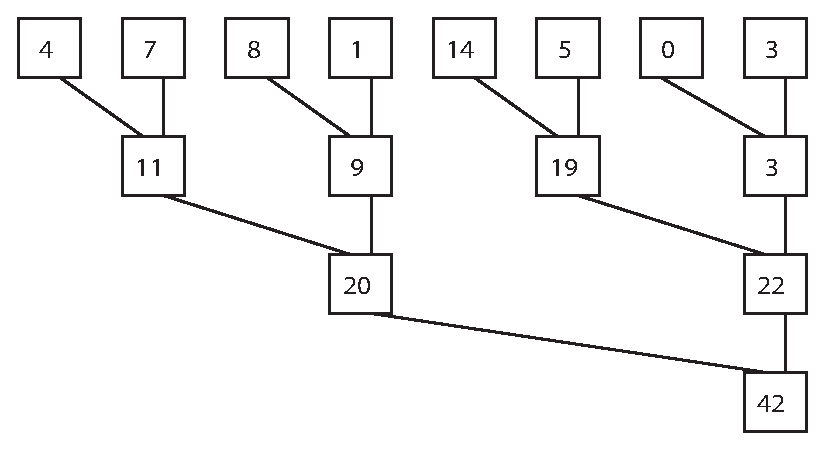
\includegraphics{parallel-left-fold-tree.pdf}
\caption{An illustration of the successive reduction of
  parallel-left-fold where $\oplus$ is set to be addition.}
\end{figure}
\vspace{1pc}

This figure is drawn with parent nodes right aligned to indicate that
the result of the addition ends up overwriting the slot originally
occupied by the second summand. The bottom-most value in each column
of the graphical representation will be the final value stored in the
temporary array that stores intermediate sums.

An explicit procedure to determine which processor performs each
$\oplus$ operation must be devised to complete this implementation of
parallel-left-fold. Note that each level in this tree represents a reduction of the original input
sequence. Since we have a balanced binary tree, the number of nodes at
the $j$th level (starting at 0) of the tree is  $\lceil \frac{n}{2^j}
\rceil$. Thus we need $\lceil \frac{n}{2^i}\rceil$ processors to
perform the $i$th (starting at 1) reduction of our sequence.
Note that there are exactly $\lceil \frac{p}{2^j} \rceil = \lceil
\frac{n}{2^{j+1}} \rceil$ numbers $l$ in the range 0 to $p-1$ for
which $(l \mod 2^j = 0)$. This means that the modulus operator can be
used, together with a variable that is multiplied by two in each
iteration to select which processors will be active. Since all $p$ of
our processors must be active in the first round, we will initialize
this variable to the value of 1. Note that this value also corresponds
to the distance between the values that each processor will add in any
particular reduction. The following pseudo-code describes the rest of
the details of the implementation.

\begin{algorithm}[h!]
\caption{parallel-left-fold where $p = n/2$ and $n=2^k$}
\begin{algorithmic}
\STATE values[pid] $\leftarrow$ input[$2\cdot \mbox{pid}$] $\oplus$ input[$2\cdot \mbox{pid} +1$]
\STATE stride $\leftarrow$ 1
\WHILE{$\mbox{pid} \mod \frac{n}{\mbox{stride}} = 0$ and $\mbox{stride} < n$}
\STATE values[pid] $\leftarrow$ values[pid] $\oplus$ values[pid $+$ stride] 
\STATE stride $\leftarrow$ stride$\cdot 2$
\ENDWHILE
\RETURN values[0]
\end{algorithmic}
\end{algorithm}

%%Since each of the computations a particular depth in the tree above are computed in lock step, the height of the tree is the running time of parallel-left fold.  Since the tree above is a balanced binary tree with $n$ leaves it has height $\lceil log_2 n \rceil$. This result can also be obtained by solving the recurrence relation (\ref{rr}) with the base case $T(1) = 0$.%%

\vspace{3pc}
\subsection{A First Attempt}

In computing parallel-left-fold in the manner described above, some of the partial sums that constitute the output of parallel-prefix-sums are computed.

\begin{figure}[h]
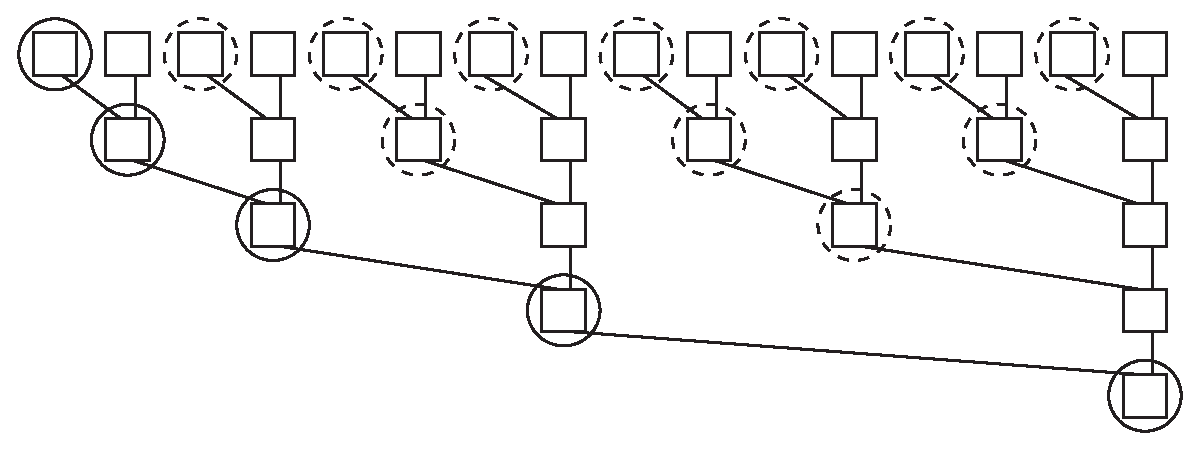
\includegraphics[scale = .75]{correctsums.pdf}
\caption{Each node in the tree that represents the final value in a slot of the temporary array is circled. A solid line indicates that the value is correct, while a dashed line indicates that the value is incorrect.}
\end{figure}
\vspace{1pc}

Specifically, all the partial sums that are placed at output indices
$2^a-1$ for positive integers $a$ are correct. The other sums that are
computed as intermediaries to the final sum are incomplete in the
sense that they are only correct prefix sums for some continuous
subsequence of the input sequence.

In general, the sum in the temporary array at the $i$th index after
the execution of parallel-left fold is the sum of the subsequence
ending at $a_i$, and including $2^j$ terms\footnote{$a_{i-(2^j-1)},
  a_{i-(2^j-1)+1}, \ldots a_i$}, where $j$ is the final round in which
that value was modified.

\begin{proof}
What we will prove is that the value at any array index $i$ that is active during the $j$th reduction is the subsequence of length $2^j$ ending at the $i$th value of the input sequence. This directly implies that the value that remains after the execution of the entire algorithm will be the value after the final reduction in which that value was changed.

We prove this claim by induction on $j$. When $j=0$ the values in the temporary array are just the values of the input sequence. Since $j=0$, $2^j = 1$, and indeed, the values of the input sequence are the trivial sums of length one, 

Suppose that the node $i$  is active during the $j+1$th reduction step. Then by our induction assumption, its value just before that reduction step is executed is the correct subsequence of length $2^j$. Similarly, the array value that is to be added to our value was also active at the $j$th reduction

\footnote{The value at the $z$th array index is active in the $j+1$th
  round when $z+1 \mod 2^{j+1} = 0$ (and $z \neq 0$). Thus $z - 2^j +
  1 = 0 \mod 2^j$, since both $z+1$ and $2^j = 0 \mod 2^j$. This is
  the index of the value on the left hand side of the $\oplus$
  operation.}

, and so its subsequence is the $\oplus$ of the sequence of length
$2^j$ ending at that index. As noted in the previous section, the
distance between terms added in the $j$th reduction is always $2^j$,
which means that these two sequences have no overlapping terms, and no
missing terms in between them. By the associativity of the operator
that is being used, the value that results from applying $\oplus$ to
these two terms is value of the subsequence ending at the rightmost index of length $2^j + 2^j = 2 \cdot 2^j = 2^{j+1}$.
\end{proof}

With this fact in hand, it is easy to determine which array indices
contain correct values. Since the value at the $i$th index of the
array is correct when it contains the $\oplus$ of the $i$ terms, any
index $i$ for which $i+1 = \max \{ 2^a : i+1 \mod 2^a = 0 \}$ will contain
a correct value. It is easy to see that this condition is only
satisfied when $i+1 = 2^a$ for some $a$.

\begin{algorithm}[h!]
\caption{parallel-prefix-sums where $p = n/2$ and $n=2^k$}
\begin{algorithmic}
\STATE output[pid] $\leftarrow$ input[$2\cdot \mbox{pid}$] $\oplus$
\STATE stride $\leftarrow$ 1
\WHILE{$\mbox{pid} \mod \frac{n}{\mbox{stride}} = 0$ and $\mbox{stride} < n$}
\STATE values[pid] $\leftarrow$ values[pid] $\oplus$ values[pid $+$ stride] 
\STATE stride $\leftarrow$ stride$\cdot 2$
\ENDWHILE
\RETURN

\STATE myitem $\leftarrow$ pid $\cdot 2$ 
\STATE segmentsize $= n/2$
\WHILE{stride $> 0$}
\IF{myitem $\mod$ segmentsize $= 0$ and pid $!=$ 0}
\STATE values[myitem -1 + segmentsize/2] += values[myitem-1]
\ENDIF
\STATE segmentsize = segmentsize/2

\ENDWHILE
\end{algorithmic}
\end{algorithm}
	
\chapter*{Conclusion}
         \addcontentsline{toc}{chapter}{Conclusion}
	\chaptermark{Conclusion}
	\markboth{Conclusion}{Conclusion}
	\setcounter{chapter}{4}
	\setcounter{section}{0}
	

    \appendix
      \chapter{The First Appendix}



  \backmatter 

    \bibliographystyle{bsts/mla-good} % there are a variety of styles available; 
    \nocite{*}
    \bibliography{thesis}
\end{document}
